\definecolor{cobaltblue}{HTML}{0047AB}
\definecolor{techgray}{HTML}{4A4A4A}

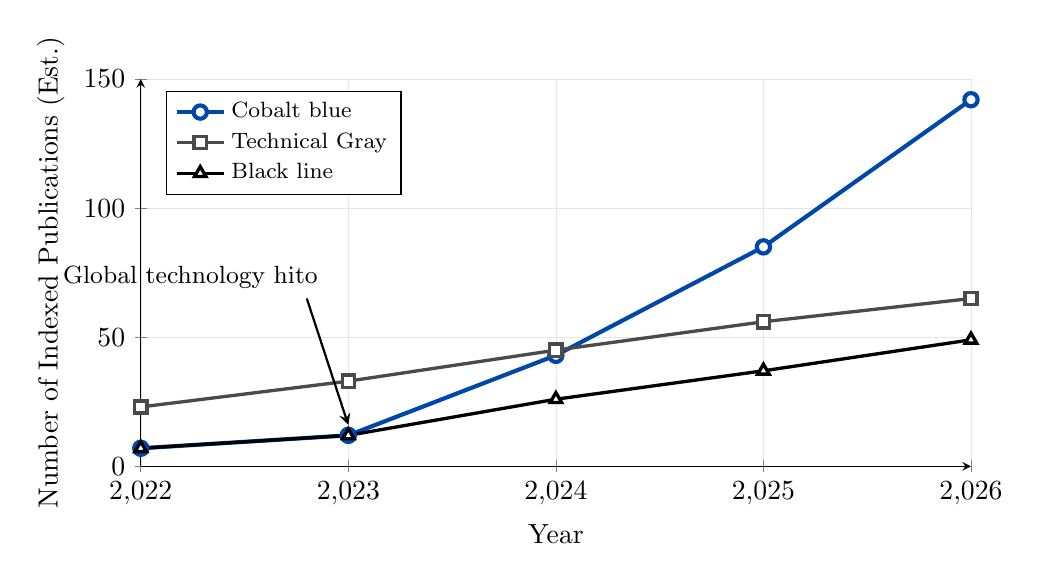
\begin{tikzpicture}
\begin{axis}[
    width=\linewidth,
    height=6.5cm,
    grid=major,
    grid style={line width=.1pt, draw=gray!20},
    xlabel={Year},
    ylabel={Number of Indexed Publications (Est.)},
    xmin=2022, xmax=2026,
    ymin=0, ymax=150,
    xtick={2022, 2023, 2024, 2025, 2026},
    ytick={0, 50, 100, 150},
    tick pos=left,
    xtick align=inside,
    ytick align=inside,
    legend pos=north west,
    % SE ELIMINÓ 'fancybox=false' PARA EVITAR EL ERROR DE COMPILACIÓN
    legend style={draw=black, fill=white, font=\footnotesize, cells={anchor=west}},
    axis x line=bottom,
    axis y line=left,
    clip=false
]

% Serie Cobalt Blue
\addplot[cobaltblue, line width=1.5pt, mark=*, mark options={fill=white, line width=1.5pt, scale=1.2}] coordinates {(2022,7)(2023,12)(2024,43)(2025,85)(2026,142)};
\addlegendentry{Cobalt blue}

% Serie Technical Gray
\addplot[techgray, line width=1.2pt, mark=square*, mark options={fill=white, line width=1.2pt, scale=1.1}] coordinates {(2022,23)(2023,33)(2024,45)(2025,56)(2026,65)};
\addlegendentry{Technical Gray}

% Serie Black Line
\addplot[black, line width=1.2pt, mark=triangle*, mark options={fill=white, line width=1.2pt, scale=1.2}] coordinates {(2022,7)(2023,12)(2024,26)(2025,37)(2026,49)};
\addlegendentry{Black line}

% Flecha y etiqueta de hito tecnológico
\draw[->, >=stealth, black, thick] (axis cs:2022.8, 65) -- (axis cs:2023, 16);
\node[black, font=\small, anchor=south east] at (axis cs:2022.9, 65) {Global technology hito};

\end{axis}
\end{tikzpicture}